%===============================================================
%   Requirements Specification
%===============================================================

\documentclass[parskip=full]{scrartcl}
\usepackage[utf8]{inputenc} % use utf8 file encoding for TeX sources
\usepackage[T1]{fontenc} % avoid garbled Unicode text in pdf
\usepackage{hyperref} % detailed hyperlink/pdf configuration
\usepackage{csquotes} % provides \enquote{} macro for "quotes"
\usepackage{graphicx} % embed graphics
\usepackage[makeindex]{glossaries}
\makeglossaries

% definitions
\newcommand{\pseAuthors}{authors here (TBD)} 
\newcommand{\pseTitle}{Project Name (TBD)}
\newcommand{\pseDocTitle}{Requirements Specification}

\hypersetup{ % ‘texdoc hyperref‘ for options
pdftitle={\pseDocTitle},
pdfauthor={\pseAuthors}}
\title{%
    \pseTitle \\
    \large \pseDocTitle}
\author{\pseAuthors}
\date{\today}

% BEGIN DOCUMENT
\begin{document}

\begin{titlepage}
\maketitle
\end{titlepage}

\tableofcontents

\section{Product Overview}

 {\pseProjectName} is a web-tool that enables its users to create, edit and manage machine learning models on different sensor data. The web-tool consists of two primary components:

\begin{enumerate}
    \item A server application that handles the API calls. Main functions of the server are handling the feature extraction, feature preprocessing, model training and managing the database.
    \item Desktop and mobile client applications to manage and interact with the models, e.g. adding new data samples, identifying given data samples and setting parameters for model training. A model can be utilized on different clients at the same time. Clients have different capabilites depending on the platform, mobile clients allow input of new data samples in form of raw sensor data, while desktop clients allow management features.
\end{enumerate}

Both components together allow for a streamlined and easy-to-use machine learning experience for both the unexperienced and the expert.
\newpage
\section{Purpose}
TBD

\subsection{Web Client}
\subsubsection{Core criteria}
\begin{itemize}
\item TBD
\end{itemize}

\subsubsection{Optional criteria}
\begin{itemize}
\item TBD
\end{itemize}

\subsubsection{Exclusion criteria}
\begin{itemize}
\item TBD
\end{itemize}


\subsection{Backend}
\subsubsection{Core criteria}
\begin{itemize}
\item TBD
\end{itemize}

\subsubsection{Optional criteria}
\begin{itemize}
\item TBD
\end{itemize}

\subsubsection{Exclusion criteria}
\begin{itemize}
\item TBD
\end{itemize}

\newpage
\section{Usage}
\subsection{Area of Application}
The application is for collecting and labeling sensor data, training a model from the collected data and serving the stored resulting model to the user to classify actions in real time.

\subsection{\textbf{Use Case Examples}}
\fbox{\parbox{\textwidth}{\label{ocfrank} Frank has sparse knowledge of machine learning. He just discovered “Explorer”. On the website that he views using his laptop, he creates a new account. After logging in, he creates a new workspace by selecting sensors to sample data (e.g., accelerometer). He sets up some simple labels (e.g. swipe right, swipe left). After opening the QR code of the workspace, he can select the action to perform on his phone from the available labels. He can also set the duration for a recorded sample and a countdown that is shown before recording. He performs some simple swipe gestures by moving his phone mid-air. The recorded data is labeled and is pushed to the laptop where he can see the data coming in. With a single click he can build a machine learning model that is immediately available on his smartphone to classify gestures.}}

\fbox{\parbox{\textwidth}{\label{ocalice} Alice is an engineer at a washing machine company. Alice has been observing that HCSOB washing machines with clogged circulating pumps show an unusual pattern of movement during the washing process (error reference 404). The washing machine is moving in a specific rhythm, which Alice recognizes when she is at the customer’s home. However, Alice would rather make a diagnosis without having to go to the customer. Then she remembers the program "Explorer" which she can use to easily develop machine learning models. With the help of the smartphone acceleration sensors in her cell phone, she and her colleagues record the movement patterns at some of her repair sites. After she has collected enough data, she can use the Explorer program to automatically train and deploy a machine learning model with one click. When a new case comes in, Alice just sends the customer a URL to a website of the Explorer. The customer places his smartphone on the washing machine and the model can determine directly "on the edge" whether error 404 is present. This saves Alice money and time. Alice can order the parts for repair and perform the repair with a single visit.}}

\subsection{Target Groups}
The target group of this application is people that wants to create a machine learning model from mobile sensor data.
That includes:
\begin{itemize}
    \item People like \hyperref[ocfrank]{Frank}, who are new to machine learning and want an easy tool to discover machine learning and create models that they can use.
    \item Experienced engineers that have knowledge of machine learning but need a fast tool to collect data and create a model.
\end{itemize}
We assume a rather technical audience. %(eloborate maybe)

\subsection{Operating Conditions}
The tool is a web application that can be run on any modern browser. A web browser must be installed on the user device to view the webpage. The application can be used from anywhere with a decent network connection.

Service Duration: 24 hours a day
\newpage
\section{Operating Environment}
Database and the server appliance both run on a server, whereas different web browsers may be used for the clients. A Docker image may be provided for the server appliance.

\subsection{Software}
\subsubsection{Server Appliance}
\begin{itemize}
    \item MongoDB support
    \item Recent versions of Node.js and Python 
\end{itemize}
\subsubsection{Client Devices}
\begin{itemize}
    \item A modern web browser (Chrome 87+, Firefox 83+) supporting: %MOBILE BROWSERS ????
    \begin{itemize}
        \item \href{https://developer.mozilla.org/en-US/docs/Web/API/Sensor_APIs}{Sensor APIs}
        \item \href{https://developer.mozilla.org/en-US/docs/Web/API/Web_Storage_API}{Web Storage API}
    \end{itemize}
\end{itemize}

\subsection{Hardware} % omer
\subsubsection{Server Appliance}
    The server has to be fast enough to support all clients. This depends on the expected number of clients. Most computations will be done on the server. \textbf{TOO ARBITRARY?}
\subsubsection{Client Devices}
\begin{itemize}
    \item \textbf{TBD}
    \item \textbf{TBD}
\end{itemize}

\newpage
\section{Functional Requirements}

\subsection{Main Functions}
These functions must be implemented in order to fulfill the core criteria.

\subsubsection{Web Client}
The web client supports both desktop and mobile modes. The functionality that will be displayed is determined by the device information of the browser.

\paragraph{Desktop Web Client}


\def\twodigits#1{%
  \ifnum#1<10 0\fi
  \number#1}

\begin{enumerate}[{label = \textbf{/F{\protect\twodigits{\arabic{enumi}}}0/}, leftmargin = *}]
    \item \label{welcome_page} Show a welcome page with a login panel when the website is accessed
    \item \label{registration_panel}Show registration panel when clicked on register in the welcome page
    \item \label{workspaces_ov}Show a workspaces overview where the available workspaces are listed after logged in
    \item Allow creating workspaces with the given name, sensors to be used and their sampling rate
    \item List the available sensors for the recordings on the workspace creation window
    \item Show the workspace panel when a workspace is selected
    \item Allow renaming workspaces on the workspace panel by double clicking on the workspace name
    \item List labels with their sample count on the labels overview window
    \item Allow creating labels for the actions to be recorded in the workspace
    \item Allow renaming labels on the labels overview
    \item Allow deleting labels which in turn deletes the data samples with the selected label
    \item Display a link to be used for recording data to the workspace when collect data is clicked
    \item Display a button to copy the link to the clipboard
    \item Display QR code with the same link in the previous function embedded to be used for recording data
    \item Display the collected data samples chronologically on the workspace panel
    \item Visualize the selected data sample as a graph when the data sample is clicked on the workspace panel 
    \item Allow changing the graph type (line plot, bar plot, box plot, histogram, distplot, heatmaps, 2D and 3D Scatter plot)
    \item Display the metadata of the selected data sample (identifier of the recording device and recording date/time)
    \item Allow setting the start/end time of the labeled actions on the graph view of the selected data sample
    \item Allow relabeling the selected data sample
    \item Allow deletion of the selected data sample
    \item Allow selecting data imputation options on the workspace panel: \\mean imputation, last observation carried forward imputation, linear or spline interpolation, moving average imputation
    \item Allow selecting feature extraction options on the workspace panel: \\min, max, variance, energy, autoregressive correlation, mean, IQR, pearson correlation, skewness, kurtosis, fourier transform
    \item Allow selecting normalization options on the workspace panel: \\MinMaxScaler, Normalizer, QuantileTransformer, RobustScaler, StandardScaler
    \item Allow selecting machine learning model on the workspace panel with the respective hyperparameters depending on the selected model: \\MLPClassifier, SVC, RandomForestClassifier, KNeighborsClassifier
    \item Request training of the model according to the selected options and automatically deploy it
    \item List trained and deployed models on the models overview
    \item Show the overview of the selected model when clicked on a model on the models overview
    \begin{itemize}
        \item \textbf{/F281/} Display the used parameters of the selected model
        \item \textbf{/F282/} Display the performance metrics of the selected model: \\Average Accuracy, Balanced Accuracy, Area under the Curve, Average Precision, Per Class Precision, Average Recall, Per Class Recall, f1-score, Per Class f1-score
    \end{itemize}
    \item Display a mini QR code symbol for each model on the models overview
    \item Display a link to use the deployed model on mobile devices when the mini QR code symbol is clicked
    \item Display a button to copy the link to the clipboard
    \item Display QR code with the same link in the previous function embedded to be used for classifying data
    \item Display a logout button on all pages
\end{enumerate}

\paragraph{Mobile Web Client}
\begin{enumerate}[resume*]
    \item Show a list of available labels that will label the recorded data when the data collection is initiated
    \item Show an error if not all the required sensors are available in the device
    \item Allow configuring the countdown duration until the recording starts
    \item Allow configuring the recording duration
    \item Show a button to initiate the recording
    \item Show a countdown page with the current configuration on display (label, sensors used and their sampling rates)
    \item Display the sensor data in real-time as curves for each sensor on a single graph
    \item Show a recording completed page when the recording duration times out
    \item Allow discarding the last recording
    \item Allow another recording with the same configuration
    \item Allow editing configurations for the next recording
    \item Show a page for classification when the link of a model is opened
    \item Start listening to the sensor data of the mobile device right after the page is loaded
    \item Display the sensor data in real-time as curves for each sensor on a single graph
    \item Display the classified actions on the webpage in real time
    \item Allow stopping the recording
    \item Display the classified actions as a chronological list when the recording is stopped
    \item Allow restarting the recording
\end{enumerate}

\subsubsection{Server API}
\begin{enumerate}[resume*]
    \item Serve authentication services
    \item Serve workspace information for a user
    \item Serve data set information for a workspace
    \item Edit the label time frames of a data sample
    \item Relabel data sample
    \item Delete data sample
    \item Create labels on a workspace
    \item Rename labels on a workspace
    \item Delete labels on a workspace (which deletes the associated data samples as well)
    \item Serve label information to the mobile client
    \item Accept data from the mobile client
    \item Initiate the configured model training
    \item Serve the model information on a workspace
    \item Rename models on a workspace
    \item Delete models on a workspace
\end{enumerate}

\subsection{Extending Functions}
\begin{enumerate}[resume*]
    \item Serve a "Stay Signed In" functionality on the desktop web client
    \item Add captcha to login after 5 consecutive failed login attempts
    \item Show a sign if a data collecting device is currently active
    \item Allow listing samples by label on the workspace panel
    \item Allow adding descriptions to the labels to assist data collection
    \item \label{/F480/} Give the user non-visual feedback if an action is identified
    \item Set a sound feedback to play when an action is identified
    \item Serve a list of languages for the user interface
    \item Support magnetometer sensor
\end{enumerate}
\newpage
\section{Data}
\subsection{System Data}
\begin{enumerate}[{label = \textbf{/D{\protect\twodigits{\arabic{enumi}}}0/}, leftmargin = *}]
    \item Source code   %delet this ?
    \item Documentation %delet this ?
    \item Webpage HTML files
    \item Webpage style sheets
    \item Webpage image files
    \item Webpage sound files (Needed only if the corresponding extending criteria \hyperref[/F480/]{F480} is fulfilled)
\end{enumerate}

\subsection{User Data}
\begin{enumerate}[resume*]
    \item User credentials
    \item Workspace information of each user
    \item Data samples of the workspaces
    \item Trained models of the workspaces
\end{enumerate}

\newpage
\section{Nonfunctional Requirements}
\subsection{Usability}
\begin{itemize}
    \item /N010/ User needs to register to use the web-tool.
    \item /N020/ Once logged in, the user should be able to record a new sample in less than 5 interactions.
    \item /N030/ Usage of the web-tool is self explanatory.
    \item /N040/ Users should be able to train and deploy the machine learning model with a single click.
\end{itemize}
\subsection{Swiftness}
\begin{itemize}
    \item /N050/ Initial page load takes under 5 seconds.
    \item /N060/ Consecutive accesses load under 1 second.
\end{itemize}
\subsection{Maintainability}
\begin{itemize}
    \item /N070/ Codebase is well documented to ease bug fixes.
    \item /N080/ Test coverage is more than 80 percent.
\end{itemize}
\subsection{Portability}
\begin{itemize}
    \item /N090/ Desktop web client should be functioning on browsers newer than Chrome version 87, Firefox version 83.
    \item /N091/ Mobile web client should be functioning on browsers newer than Chrome version 87, Firefox version 83.
\end{itemize}
\subsection{Security}
\begin{itemize}
    \item /N100/ A workspace is inaccessible to other users without the QR code or the link to the workspace.
\end{itemize}
\subsection{Scalability}
\begin{itemize}
    \item /N110/ A maximum of 500 workspaces with a maximum of 100 users at the same time is supported. 
\end{itemize}

\newpage
\section{System Models}
In the following possible use cases for {\pseProjectName} are listed and the first-usage case is explained using a sequence diagramm. Control flow for different clients are given as flowcharts under Desktop and Mobile system models.

\subsection{Use Cases} \label{Use Cases}
\subsubsection{First-Usage Use Case}
This use case shows a possible usage of the application by a first time user, Frank.

\fbox{\parbox{\textwidth}{\label{ocfrank} Frank has sparse knowledge of machine learning. He just discovered “Explorer”. On the website that he views using his laptop, he creates a new account. After logging in, he creates a new workspace by selecting \glspl{sensor} to sample data (e.g., \gls{accelerometer}). He sets up some simple labels (e.g. swipe right, swipe left). After opening the QR code of the workspace, he can select the action to perform on his phone from the available labels. He can also set the duration for a recorded sample and a countdown that is shown before recording. He performs some simple swipe gestures by moving his phone mid-air. The recorded data is labeled and is pushed to the laptop where he can see the data coming in. With a single click he can build a machine learning model that is then available on his smartphone after scanning it's QR code to classify gestures.}}

\newpage

\subsubsection{Enterprise Use Case}
This use case shows a possible usage by a HCSOB employee, Alice, using the application to assist customers.

\fbox{\parbox{\textwidth}{\label{ocalice} Alice is an engineer at a washing machine company. Alice has been observing that HCSOB washing machines with clogged circulating pumps show an unusual pattern of movement during the washing process (error reference 404). The washing machine is moving in a specific rhythm, which Alice recognizes when she is at the customer’s home. However, Alice would rather make a diagnosis without having to go to the customer. Then she remembers the program "Explorer" which she can use to easily develop machine learning models. With the help of the smartphone acceleration \glspl{sensor} in her cell phone, she and her colleagues record the movement patterns at some of her repair sites. After she has collected enough data, she can use the Explorer program to automatically train and deploy a machine learning model with one click. When a new case comes in, Alice just sends the customer a URL to a website of the Explorer. The customer places his smartphone on the washing machine and the model can determine directly "on the edge" whether error 404 is present. This saves Alice money and time. Alice can order the parts for repair and perform the repair with a single visit.}}

\subsubsection{Non-Enterprise Use Case}
This use case shows a possible usage by a small business in the context of a personal trainer, Brandon, using the application to improve and expand his business model.

\fbox{\parbox{\textwidth}{\label{oc} Brandon is a body building trainer in a big metropol. He has been training people for many years but the latest Covid-21 virus hit his business hard as he couldn't assist people anymore. He recently watched an advert about the Explorer app and had this wonderful idea that would allow him train customers remotely and earning money in these trying times. He opened the Explorer app, made himself an account and created labels for his custom exercise routines. After all, he had developed many creative exercise techniques as an experienced body builder. He sent the QR code to his old students that had mastered his techniques to collect diverse samples. With one simple click, he trained a succesful model with the default options. He contected people and asked them to try his new business model. He sent the link to his model to them and with precise instructions for each exercise. With the help of his trained model, people received a feedback in real time if they were performing the exercise routines correctly. }}

\subsection{Main Functionality}
This sequence diagramm explores the first usage use case given in the previous section in detail. 

\begin{center}
    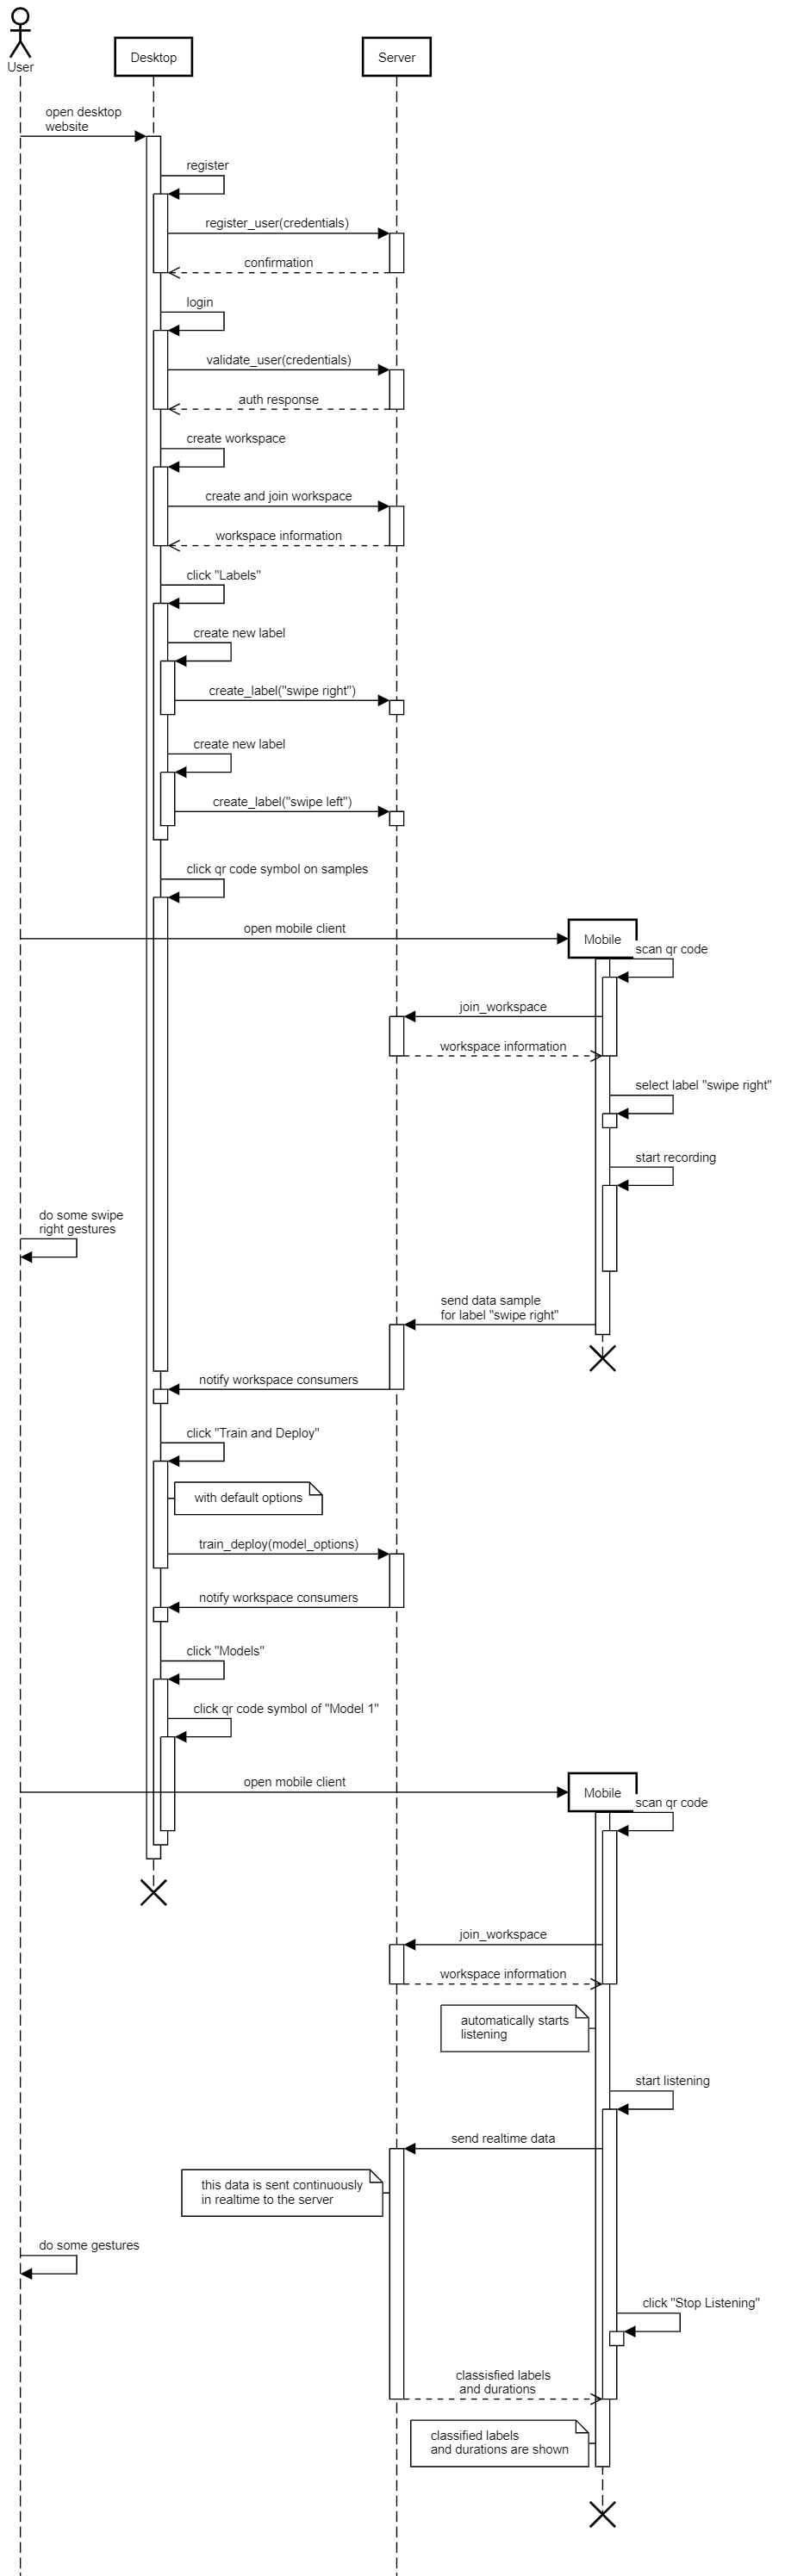
\includegraphics[width=\textwidth,trim={0 66cm 0 0},clip]{charts/sequencefrank.png}
\end{center}
\begin{center}
    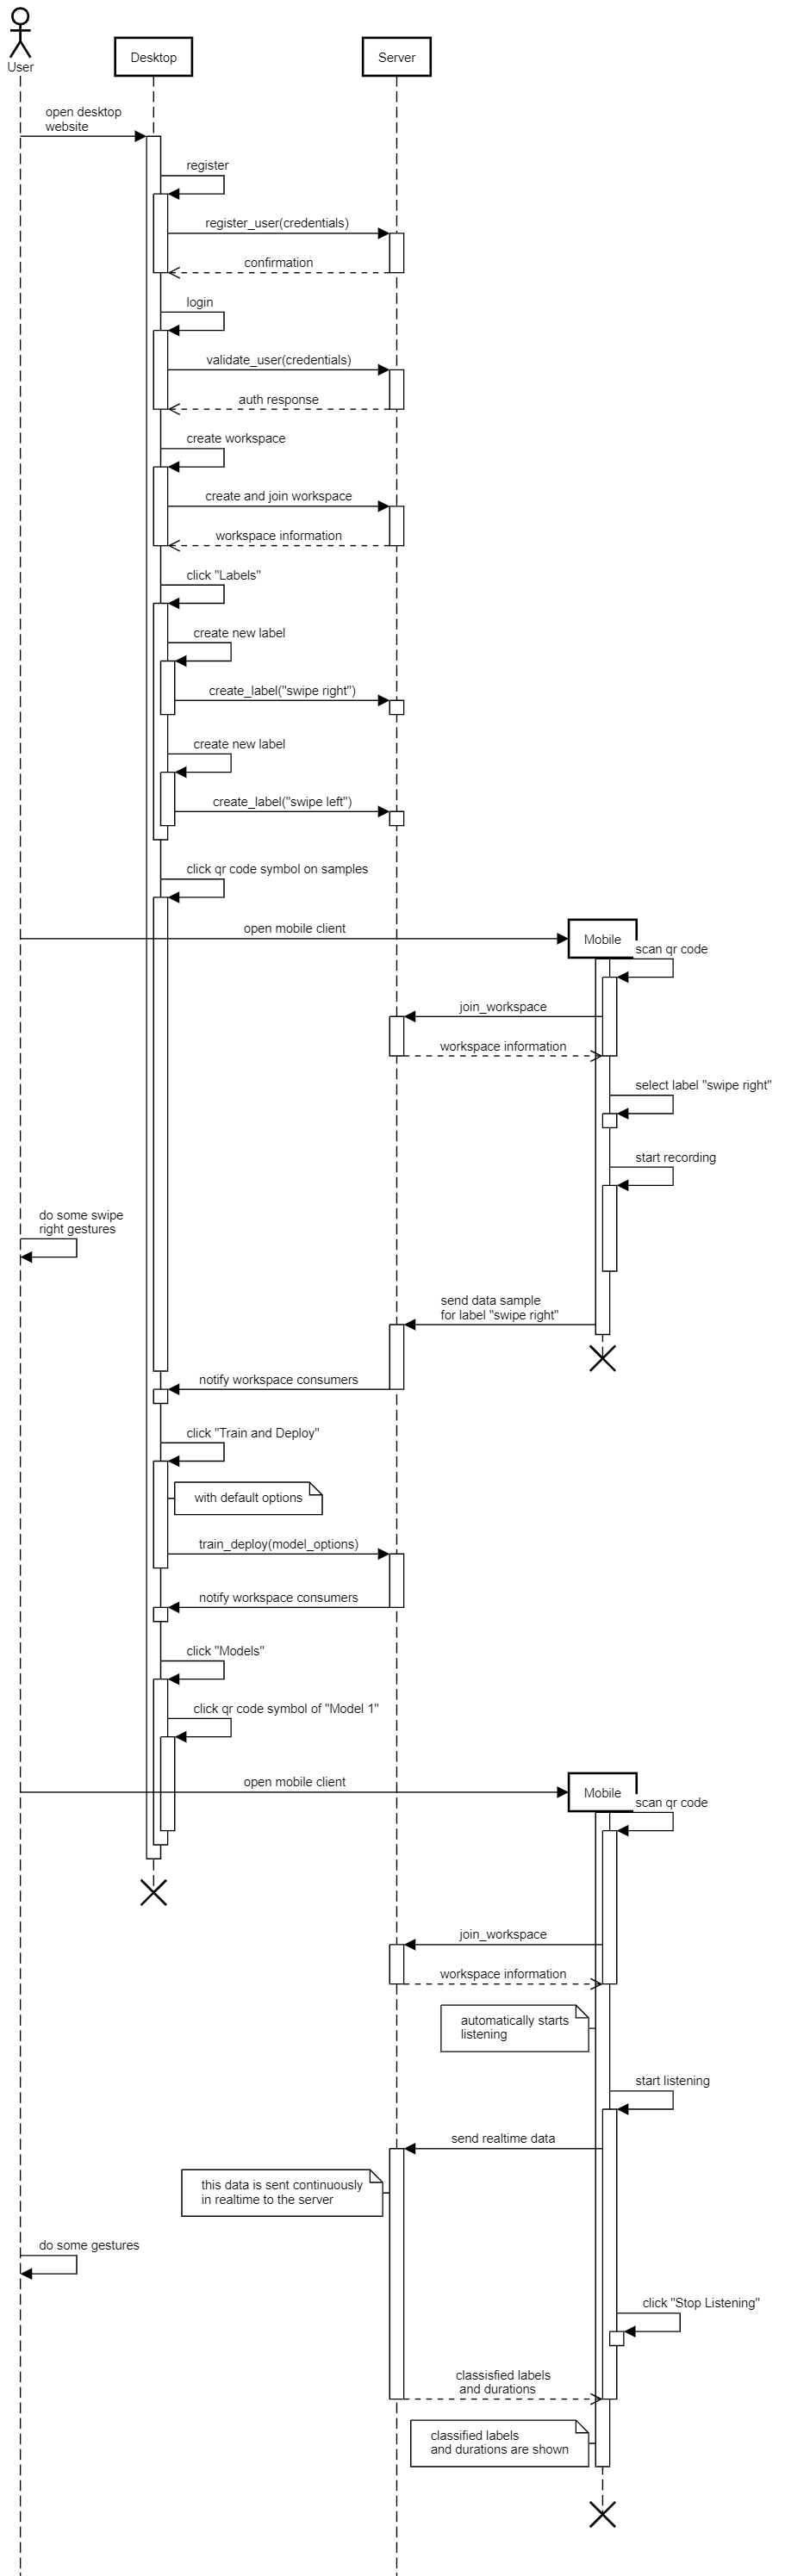
\includegraphics[width=\textwidth,trim={0 23cm 0 37cm},clip]{charts/sequencefrank.png}
\end{center}
\begin{center}
    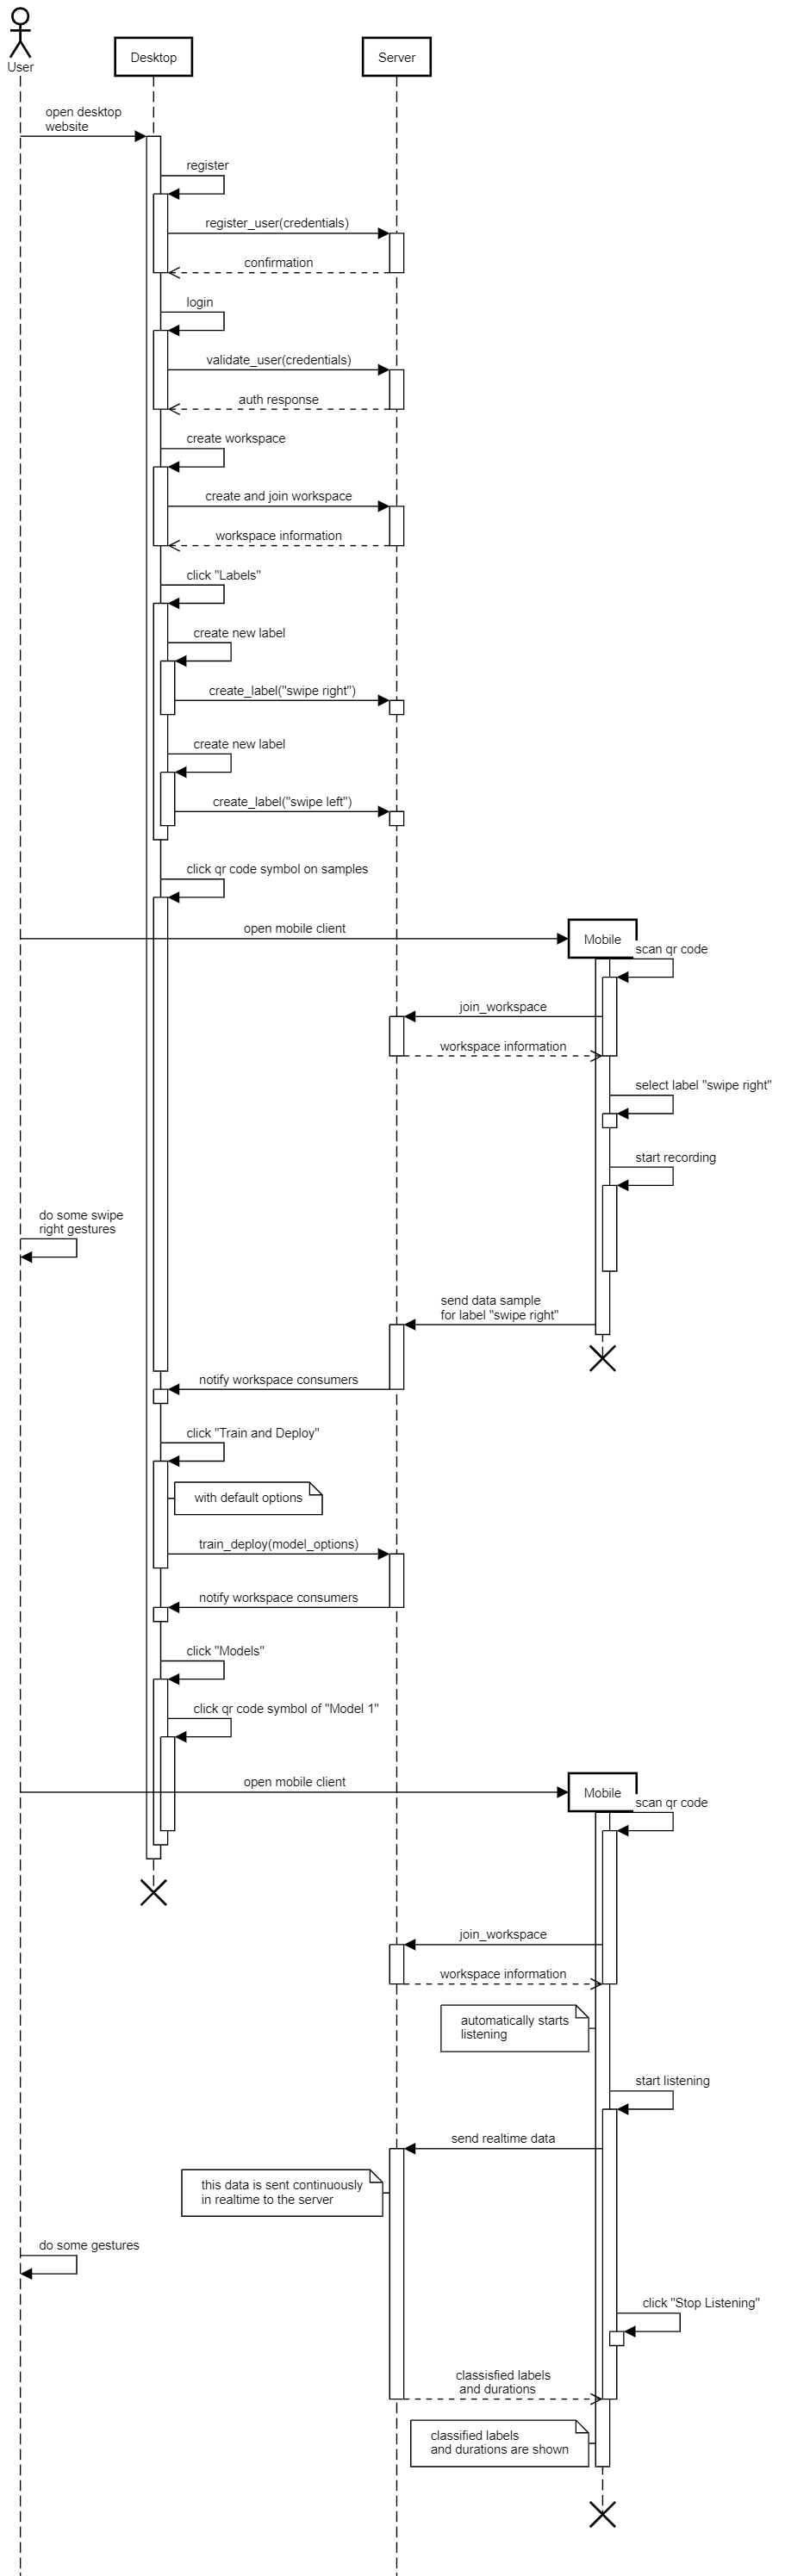
\includegraphics[width=\textwidth,trim={0 0 0 72cm},clip]{charts/sequencefrank.png}
\end{center}

\newpage
\subsection{Desktop System Model}
Following flowchart illustrates the control flow of the desktop client. 
\begin{center}
    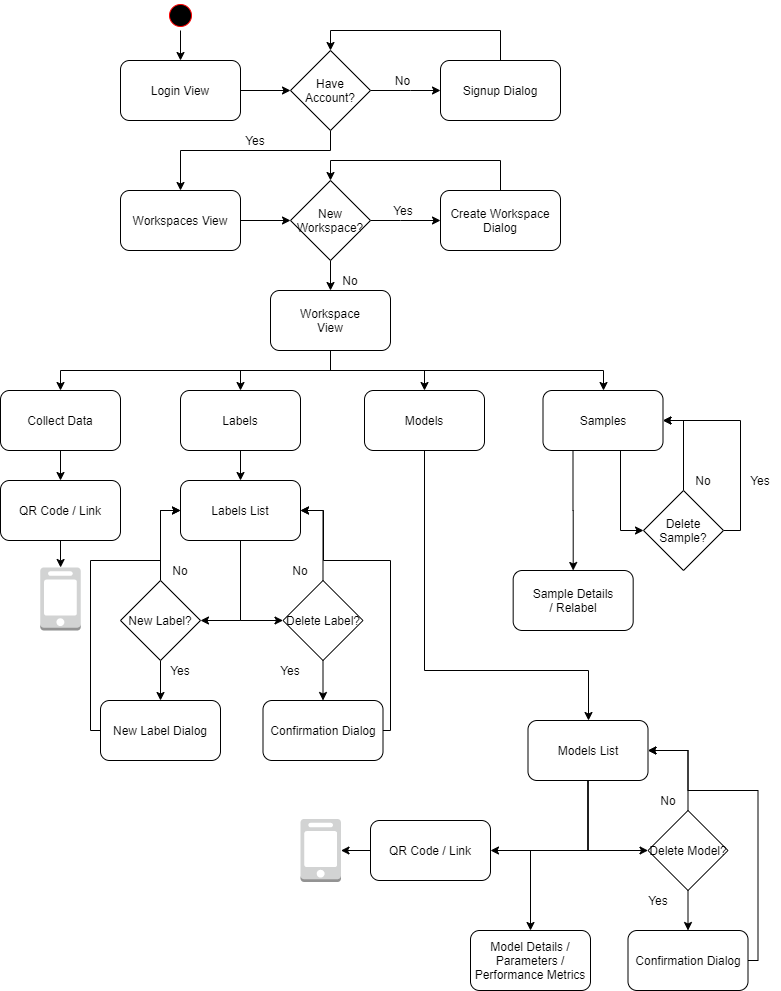
\includegraphics[width=\textwidth,height=0.85\textheight,keepaspectratio]{charts/flow1.png}
\end{center}

\newpage

\subsection{Mobile System Model}
Following flowcharts illustrate the control flow of the mobile clients. 
\vspace{1cm}

\begin{figure}[h!]
    \begin{minipage}{0.5\textwidth}
        \centering
        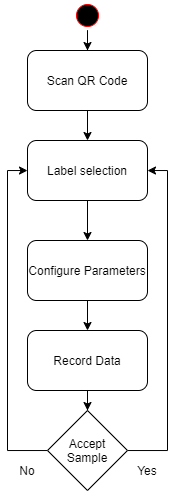
\includegraphics[width=.8\textwidth]{charts/flow2.png}
        \caption{Data Entry}
    \end{minipage}
    \begin{minipage}{0.5\textwidth}
        \centering
        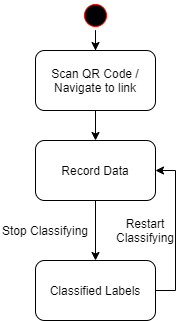
\includegraphics[width=.8\textwidth]{charts/flow3.png}
        \caption{Classification}
    \end{minipage}
\end{figure}
\newpage
\section{User Interface}
The user interface of both the desktop and mobile client will be designed so that a user without a lot of technical knowledge of machine learning can easily make use of this web-tool. The user interface is also great for experienced engineers as it presents a simple and fast way to create models and start classifying data right away.

\subsection{Desktop}
The users are first met with a simple \hyperref[fig:login]{login/registration panel}. Then the \hyperref[fig:workspaces-list]{current workspaces} are listed, from which the users can choose to work with. The users can also \hyperref[fig:create-workspace]{create a new workspace}, in which they name it and choose the labels it will have. In the \hyperref[fig:workspace-overview]{workspace overview} page, the collected data samples are listed on the left, and on the right there are buttons to view the labels and models. The users can also easily select hyperparameters and train and deploy a model in this page with a single click.\hyperref[fig:workspace-link]{A link and a QR code}, which a mobile web client can use to start collecting data to this workspace, will also be available with a single click. Users can also see the \hyperref[fig:sample-overview]{data sample overview}, \hyperref[fig:labels-overview]{labels overview} and the \hyperref[fig:models-overview]{models overview}. Each model will provide \hyperref[fig:model-link]{its own link and QR code}, which a mobile client can use to start classifying actions with this mode and which again will be provided with a single click.

\subsection{Mobile}
When a QR Code is scanned or a link is visited, the users are met with a list of labels to choose from. When a label is selected, users are allowed to configure the recording parameters before pressing the button to start recording. After that, the countdown runs and then the recording page is displayed. In the end, it is stated that the recording is done. The users can repeat the recording process by pressing a redo button in this page or discard the previous recording.

Details of the mobile web client can be seen in the \hyperref[fig:mobile]{screenshots}.

\newpage

\subsection{Screenshots}

\begin{figure}[ht]
    \centering
    \fbox{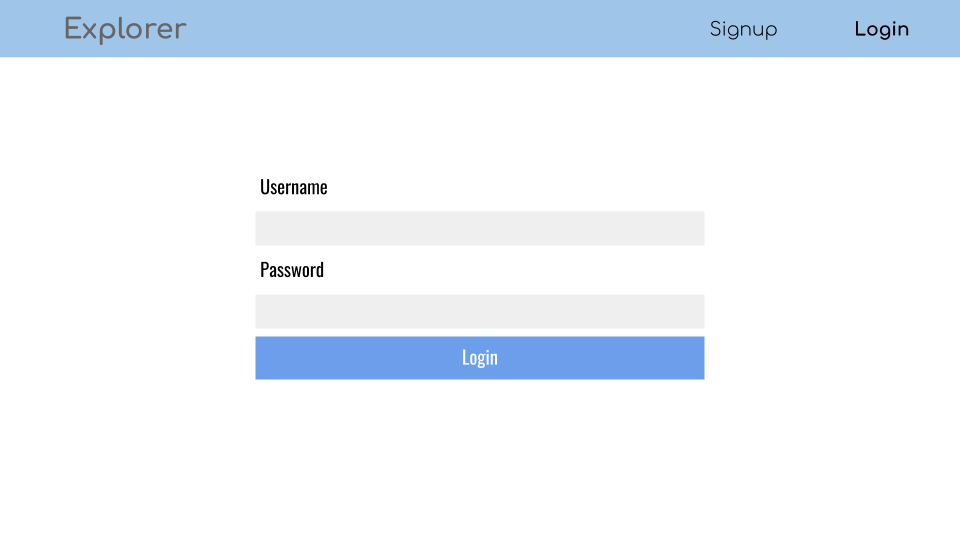
\includegraphics[width = .98\textwidth]{mockups/1.png}}
    \caption{Login/Registration Panel}
    \label{fig:login}
\end{figure}

\begin{figure}[!ht]
    \centering
    \fbox{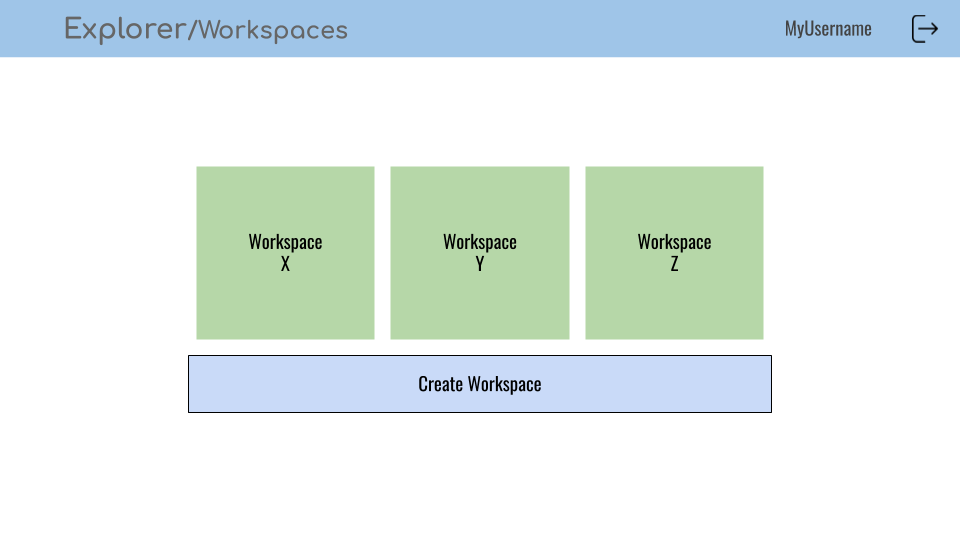
\includegraphics[width = .98\textwidth]{mockups/2.png}}
    \caption{List of current workspaces}
    \label{fig:workspaces-list}
\end{figure}

\begin{figure}[ht]
    \centering
    \fbox{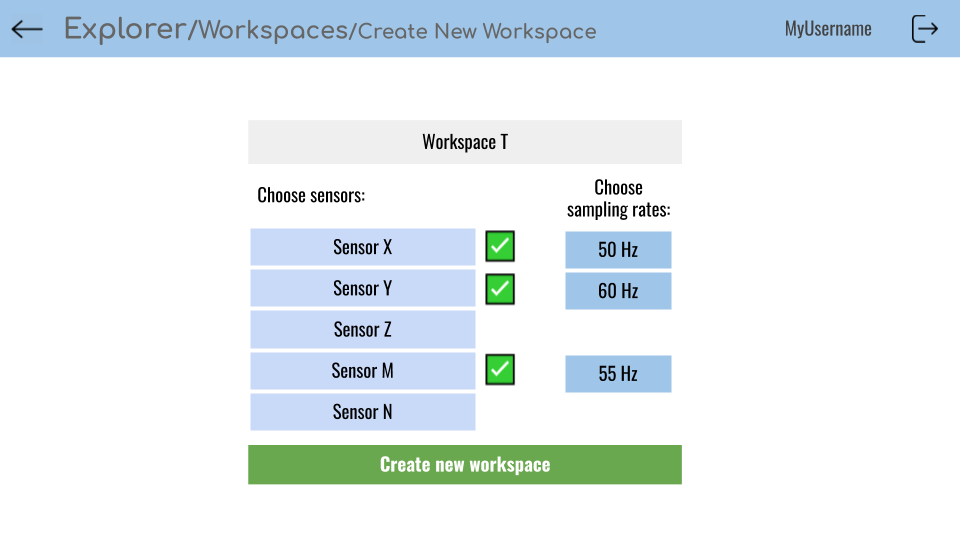
\includegraphics[width = .98\textwidth]{mockups/3.png}}
    \caption{Create a new workspace}
    \label{fig:create-workspace}
\end{figure}

\begin{figure}[ht]
    \centering
    \fbox{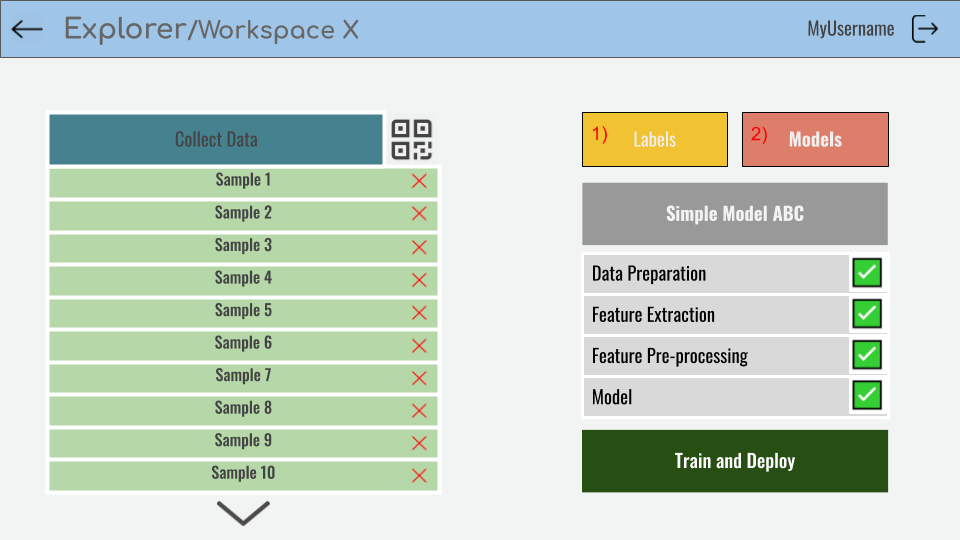
\includegraphics[width = .98\textwidth]{mockups/4.png}}
    \caption{Workspace overview}
    \label{fig:workspace-overview}
\end{figure}

\begin{figure}[ht]
    \centering
    \fbox{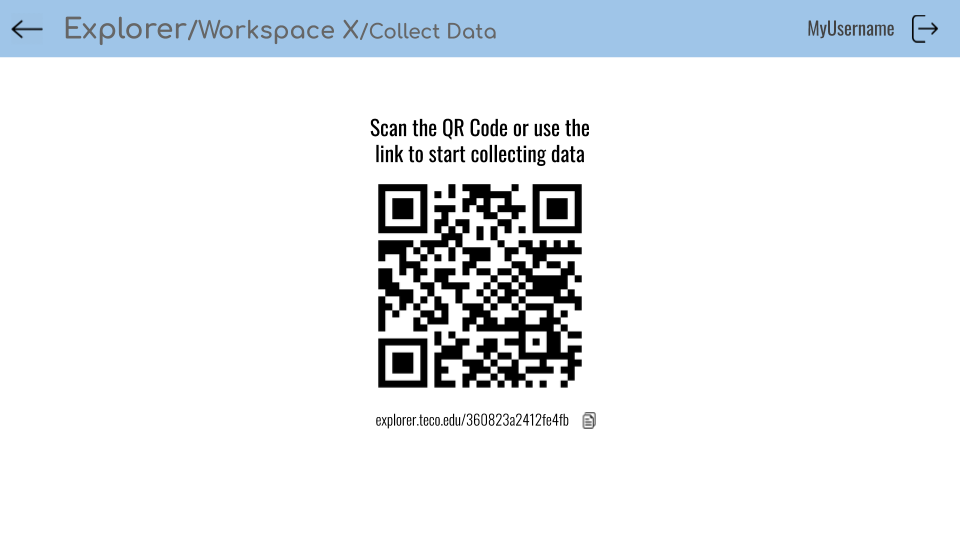
\includegraphics[width = .98\textwidth]{mockups/6.png}}
    \caption{QR Code/Link of workspace to collect data}
    \label{fig:workspace-link}
\end{figure}

\begin{figure}[ht]
    \centering
    \fbox{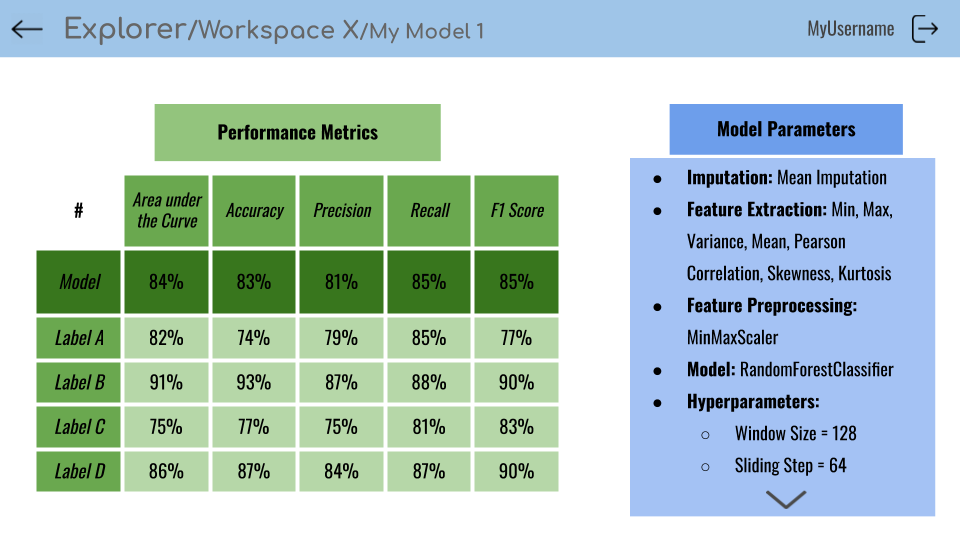
\includegraphics[width = .98\textwidth]{mockups/10.png}}
    \caption{Data sample overview}
    \label{fig:sample-overview}
\end{figure}

\begin{figure}[ht]
    \centering
    \fbox{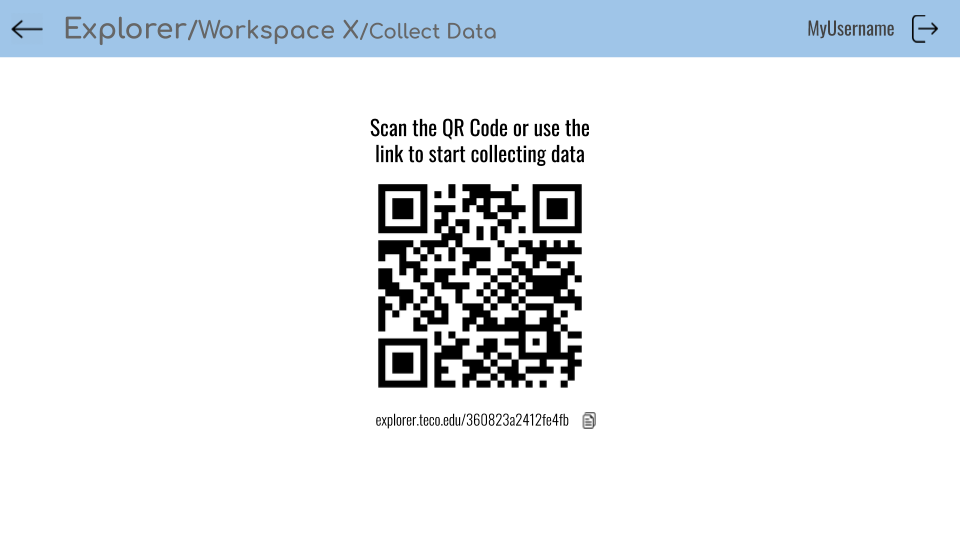
\includegraphics[width = .98\textwidth]{mockups/5.png}}
    \caption{Labels overview}
    \label{fig:labels-overview}
\end{figure}

\begin{figure}[ht]
    \centering
    \fbox{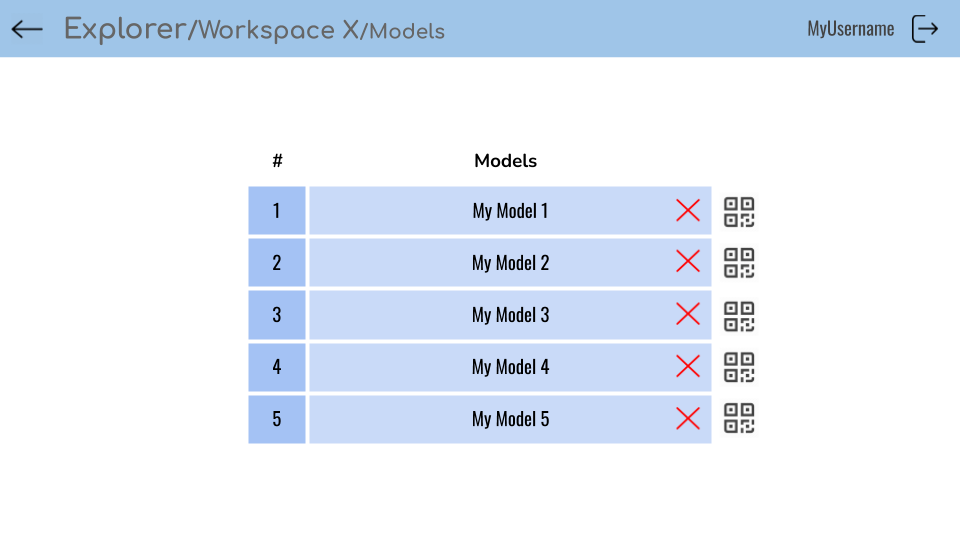
\includegraphics[width = .98\textwidth]{mockups/7.png}}
    \caption{Trained models overview}
    \label{fig:models-overview}
\end{figure}

\begin{figure}[ht]
    \centering
    \fbox{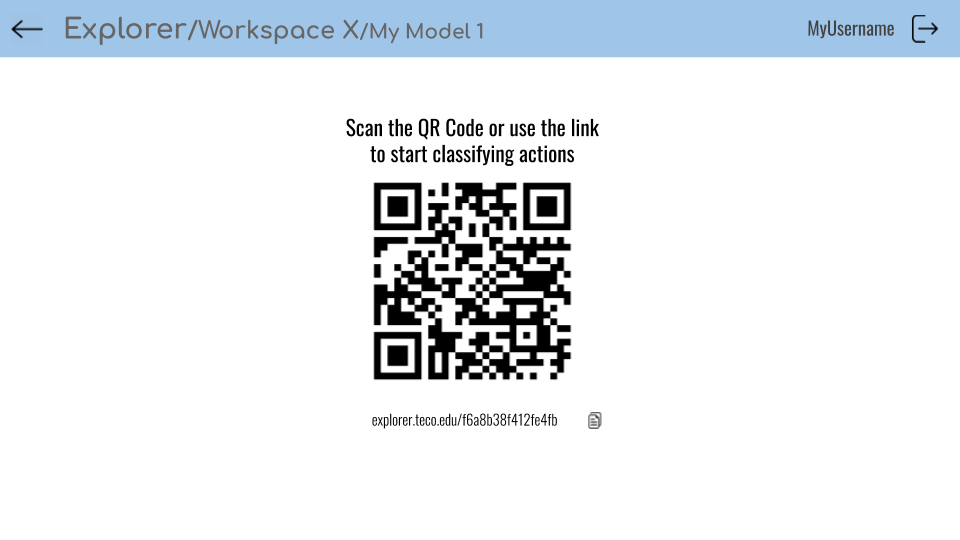
\includegraphics[width = .98\textwidth]{mockups/8.png}}
    \caption{QR Code/Link of trained model to classify data}
    \label{fig:model-link}
\end{figure}

\begin{figure}[ht]
    \centering
    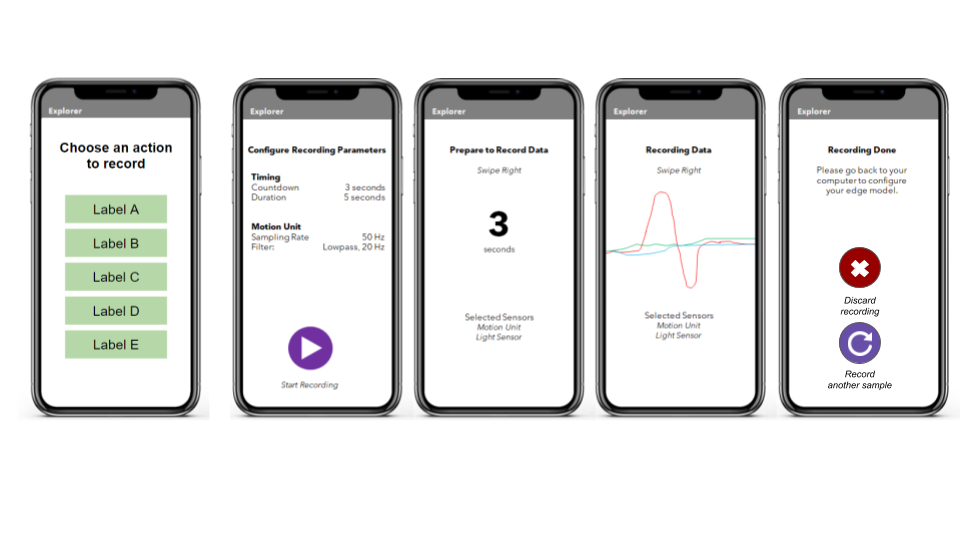
\includegraphics[width = \textwidth]{mockups/9.png}
    \caption{Data collection in mobile}
    \label{fig:mobile}
\end{figure}
\newpage

\section{??Qualitatszielbestimmung??}
\newpage

\section{Test Cases and Test Scenarios}
TBD
\subsection{Test Cases}
\subsubsection{Main Test Cases}
These test cases are necessary for the web-tool to work properly and succeed in serving
basic requests.

\begin{enumerate}[{label = \textbf{/T{\protect\twodigits{\arabic{enumi}}}0/}, leftmargin = *}]
    \item Access web page \hyperref[/F010/]{/F010/}
    \begin{itemize}
        \item \textbf{/T011/} via Google Chrome,
        \item \textbf{/T012/} via Mozilla Firefox.
    \end{itemize}
    \item Create a new user. 010, 330
    \item Login with existing credentials. 010, 330
    \item Login with invalid credentials. 010, 330
    \item Open an already existing workspace. 020, 040, 060, 340
    \item Create a new workspace. 030
    \item Rename the workspace. 050
    \item Create new label. 070
    \item Rename label. 090
    \item Delete label. 100
    \item Delete sample. 140
    \item Scan QR code. 110
    \item Open the workspace link. 110
    \item Overview collected data. 120
    \item Overview an individual data sample. 130
    \item Overview trained models. 150
    \item Overview an individual model. 160
    \item Check performance metrics of a model. 170
    \item Train and deploy a model. 190
    \item Set the duration of the recording. 220
    \item Set the sampling rate. 230
    \item Record with specified configuration. 240, 250, 260, 290, 300
    \item Overview sensor data whilst recording. 270, 280
    \item Record again with same configuration. 310
    \item Record again with different configuration. 320
\end{enumerate}
\subsubsection{Extending Test Cases}
TBD
\subsection{Test Scenarios}
The test scenarios are composed of the mentioned test cases. Starred test scenarios indicate that the scenario includes extending functionalities.
\subsubsection{Test Scenario 1 - First Time User}
A user who is new to machine learning applications opens the webpage on their computer and registers to the service. The user collects data using the default configuration with their phone and creates a machine learning model. The user then uses this model to identify new data they record. 
\newpage
\begin{enumerate}
    \item /T010/ Access web page.
    \item /T020/ Create a new user.
    \item /T030/ Login with existing credentials.
    \item /T060/ Create a new workspace.
    \item /T120/ Scan QR code.
    \item /T270/ Record with specified configuration.
    \item /T290/ Record again with same configuration.
    \item /T190/ Train and deploy a model.
\end{enumerate}
\subsubsection{Test Scenario 2 - Invalid credentials}
User tries to login with invalid credentials first and manages to login after a few unsuccessful attempts.
\begin{enumerate}
    \item /T010/ Access web page.
    \item /T030/ Login with invalid credentials.
    \item /T030/ Login with invalid credentials.
    \item /T030/ Login with existing credentials.
\end{enumerate}
\subsubsection{Test Scenario 3 - Unsupported Desktop Client}
User opens the website on an unsupported desktop browser and is welcomed with an error message.
\begin{enumerate}
    \item 
\end{enumerate} 
\subsubsection{Test Scenario 4 - Unsupported Mobile Client}
User scans the QR code they received to begin recording data. It turns out their device doesn't support the Sensor API and  
\subsubsection{Test Scenario 4 - Forgotten Password}
User tries to login with an invalid username and/or password. After a few attempts user requests a new password using the "Forgot Password" functionality and successfully manages to login using their new password.
\begin{enumerate}
    \item 
\end{enumerate} 
\subsubsection{Test Scenario 5 - Data Deletion} 
User logs in and opens their previously set workspace. User finds some data samples and labels to be improper and deletes them.
\begin{enumerate}
    \item 
\end{enumerate}
\subsubsection{Test Scenario 6 - Interruption during Recording}
User uses the link they was provided previously to start collecting data. After configuring the options the user starts the recording. Whilst recording user receives a phone call. Recording continues during the call. The user then discards the recording and start a new recording. 
\begin{enumerate}
    \item /T010/ Access web page.
    \item /
\end{enumerate}
\subsubsection{Test Scenario 7 - Registration with Already Existing Credentials}
User opens the website on their desktop device and tries to register with an already existing username.
\subsubsection{Test Scenario 8 - Multi-language Support*}
User opens the website and changes the langauge option to German. 
\subsubsection{Test Scenario 9 - Extensive Use of Main Functionalities} % better title pls
User opens the website and creates a new account. 
\subsubsection{Test Scenario 10 - Extensive Use of All Functionalities} % better title pls cuz not all, dont include edge cases, rather show relevant use case
\newpage
\section{Development Environment}
\subsection{Operating Systems}
\begin{itemize}
    \item Windows 10 with WSL1 / WSL2
    \item Ubuntu 20.04.1 LTS
\end{itemize}
\subsection{IDEs, Editors}
\begin{itemize}
    \item VS Code
\end{itemize}
\subsection{Versioning}
\begin{itemize}
    \item git
    \item Github for hosting
\end{itemize}
\subsection{Integration}
\begin{itemize} % omer
    \item \textbf{(we'll need a CI server, TECO has one?) FIXME}
\end{itemize}
\subsection{Miscallaneous}
\begin{itemize}
    \item {\LaTeX} for documents
    \item 3D Paint for mockups % paint lol?
    \item VS Code Live Share for communication
    \item Discord for communication
\end{itemize}

And many more to be added later...
\newpage

\printglossary

% END DOCUMENT
\end{document}
